\section{Archive process implementation}
This section gives an overview for the architecture of the archive process that would be responsible
to move the project data to the Synology. 

\subsection{Components for the archive process}
An Archive in the MARS ecosystem is tedious due to its distributed architecture. The process requires communication between a many components for a 
successful run. Figure \ref{fig:archiveComponent} depicts the high level components and the interfaces that the archive requires. The Archive
component exposes an API (Section \ref{section:APIDesign}) via an external port to the client. 

The marking component includes interfaces to mark a project and unmark the project in case of failure. This component communicates with the marking service which
is responsible for marking all the resources. Also, the metadata, file, scenario, result configurations, sim plans and sim runs components get make a connection to 
their respective services get the corresponding data which would be stored in the Synology using the interface provided by the Synology component.

\subsubsection{Performance optimization for simulation results}
For better performance
the simulation results are archived  using a database dump provided by the interface that will be triggered using the archive simulation result component. 
Dumping the result data directly to the Synology increases the throughput of the Archive service by reducing the network calls and decreases the total data processing
time because it has to be processed only at one end i.e. Database utility service. For this purpose a dumping API endpoint will be implemented which would trigger the data dump process in the 
Synology. In addition, it can be argued why other external components (e.g. file service) do not have a direct dependency to the Synology as it would reduce more
processing times as well. One of the main goals of the Archive service is also to act as an abstraction layer for the archives and in case of future changes the
connection interface must only be changed in inside the Archive service instead of all the other services.

\begin{figure}[H]
    \centering 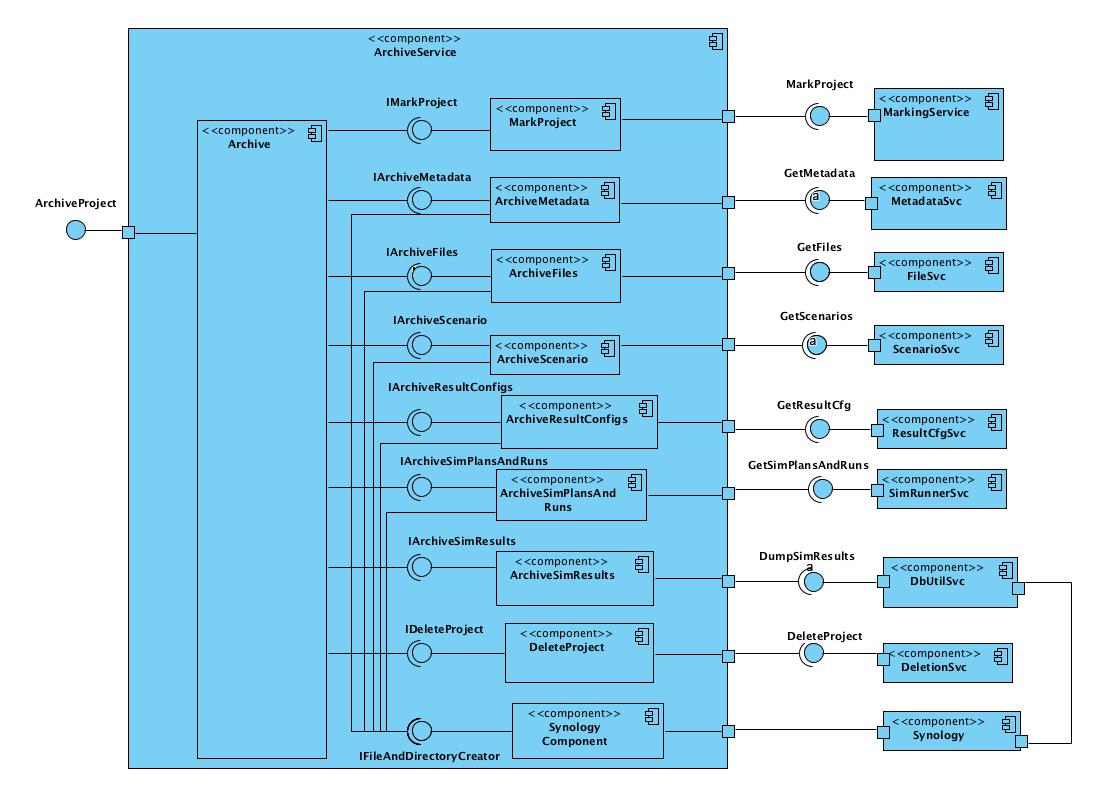
\includegraphics[scale=0.45]{grafiken/archiveComponent.png}
    \caption{Component Diagram for the Archive process}
    \label{fig:archiveComponent}
\end{figure}



\begin{figure}[H]
    \centering 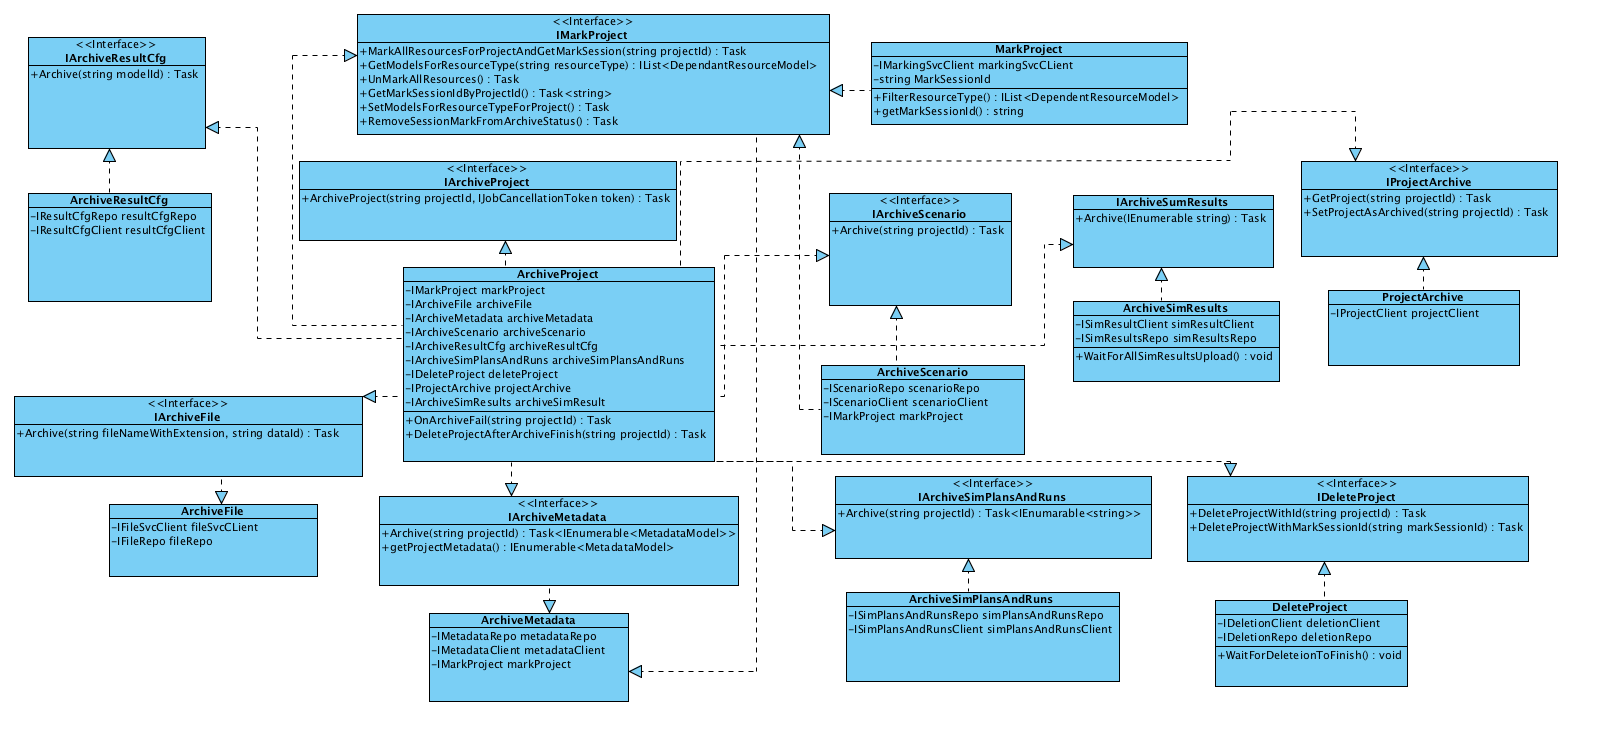
\includegraphics[height=6.5cm, angle=90, origin=c, width=11cm]{grafiken/archiveClassDiagram.png}
    \caption{Class Diagram for the Archive process}
    \label{fig:archiveClassDiagram}
\end{figure}